\section{Design-klassediagram}
\todo[inline]{Thomas A: lav diagram og forklar}
\begin{figure}[ht]
\centering
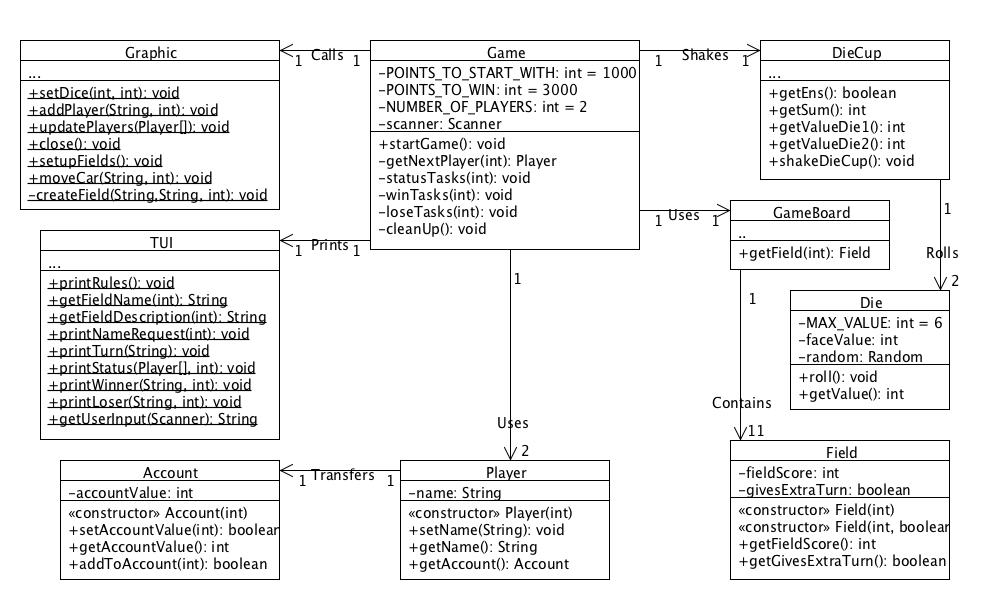
\includegraphics[scale=0.4]{DesignClass.jpg}
\caption[<Text for the list of figures>]{Design-Klassediagram}
\label{fig:figure2}
\end{figure}
Vi har også valgt at dokumentere vores program med et klassediagram. Dette giver et godt overblik over programmets opbygning, og om vi har overholdt tankegangen for \textbf{GRASP}. Denne tankegang vil blive beskrevet i næste afsnit.